\chapter{Matching}

\begin{descr}
    Matchings in undirected graphs without parallel edges and loops
\end{descr}

\section{Elementary Definitions}\index{Elementary Definitions}
\begin{definition}
A matching in an undirected (finite) graph $G=(V,E)$ is a set $M \subseteq E$ such that no two edges share a node.
A matching $M$ is called \emph{maximal} if, for any matching $M'$ with $M \subseteq M'$, $M=M'$ holds.
$M$ is of maximum cardinality if $\lvert M \rvert \ge \lvert M' \rvert $ for any matching $M'$. $M$ is \emph{perfect}
if every node is incident on one edge.
\end{definition}

\begin{example*}
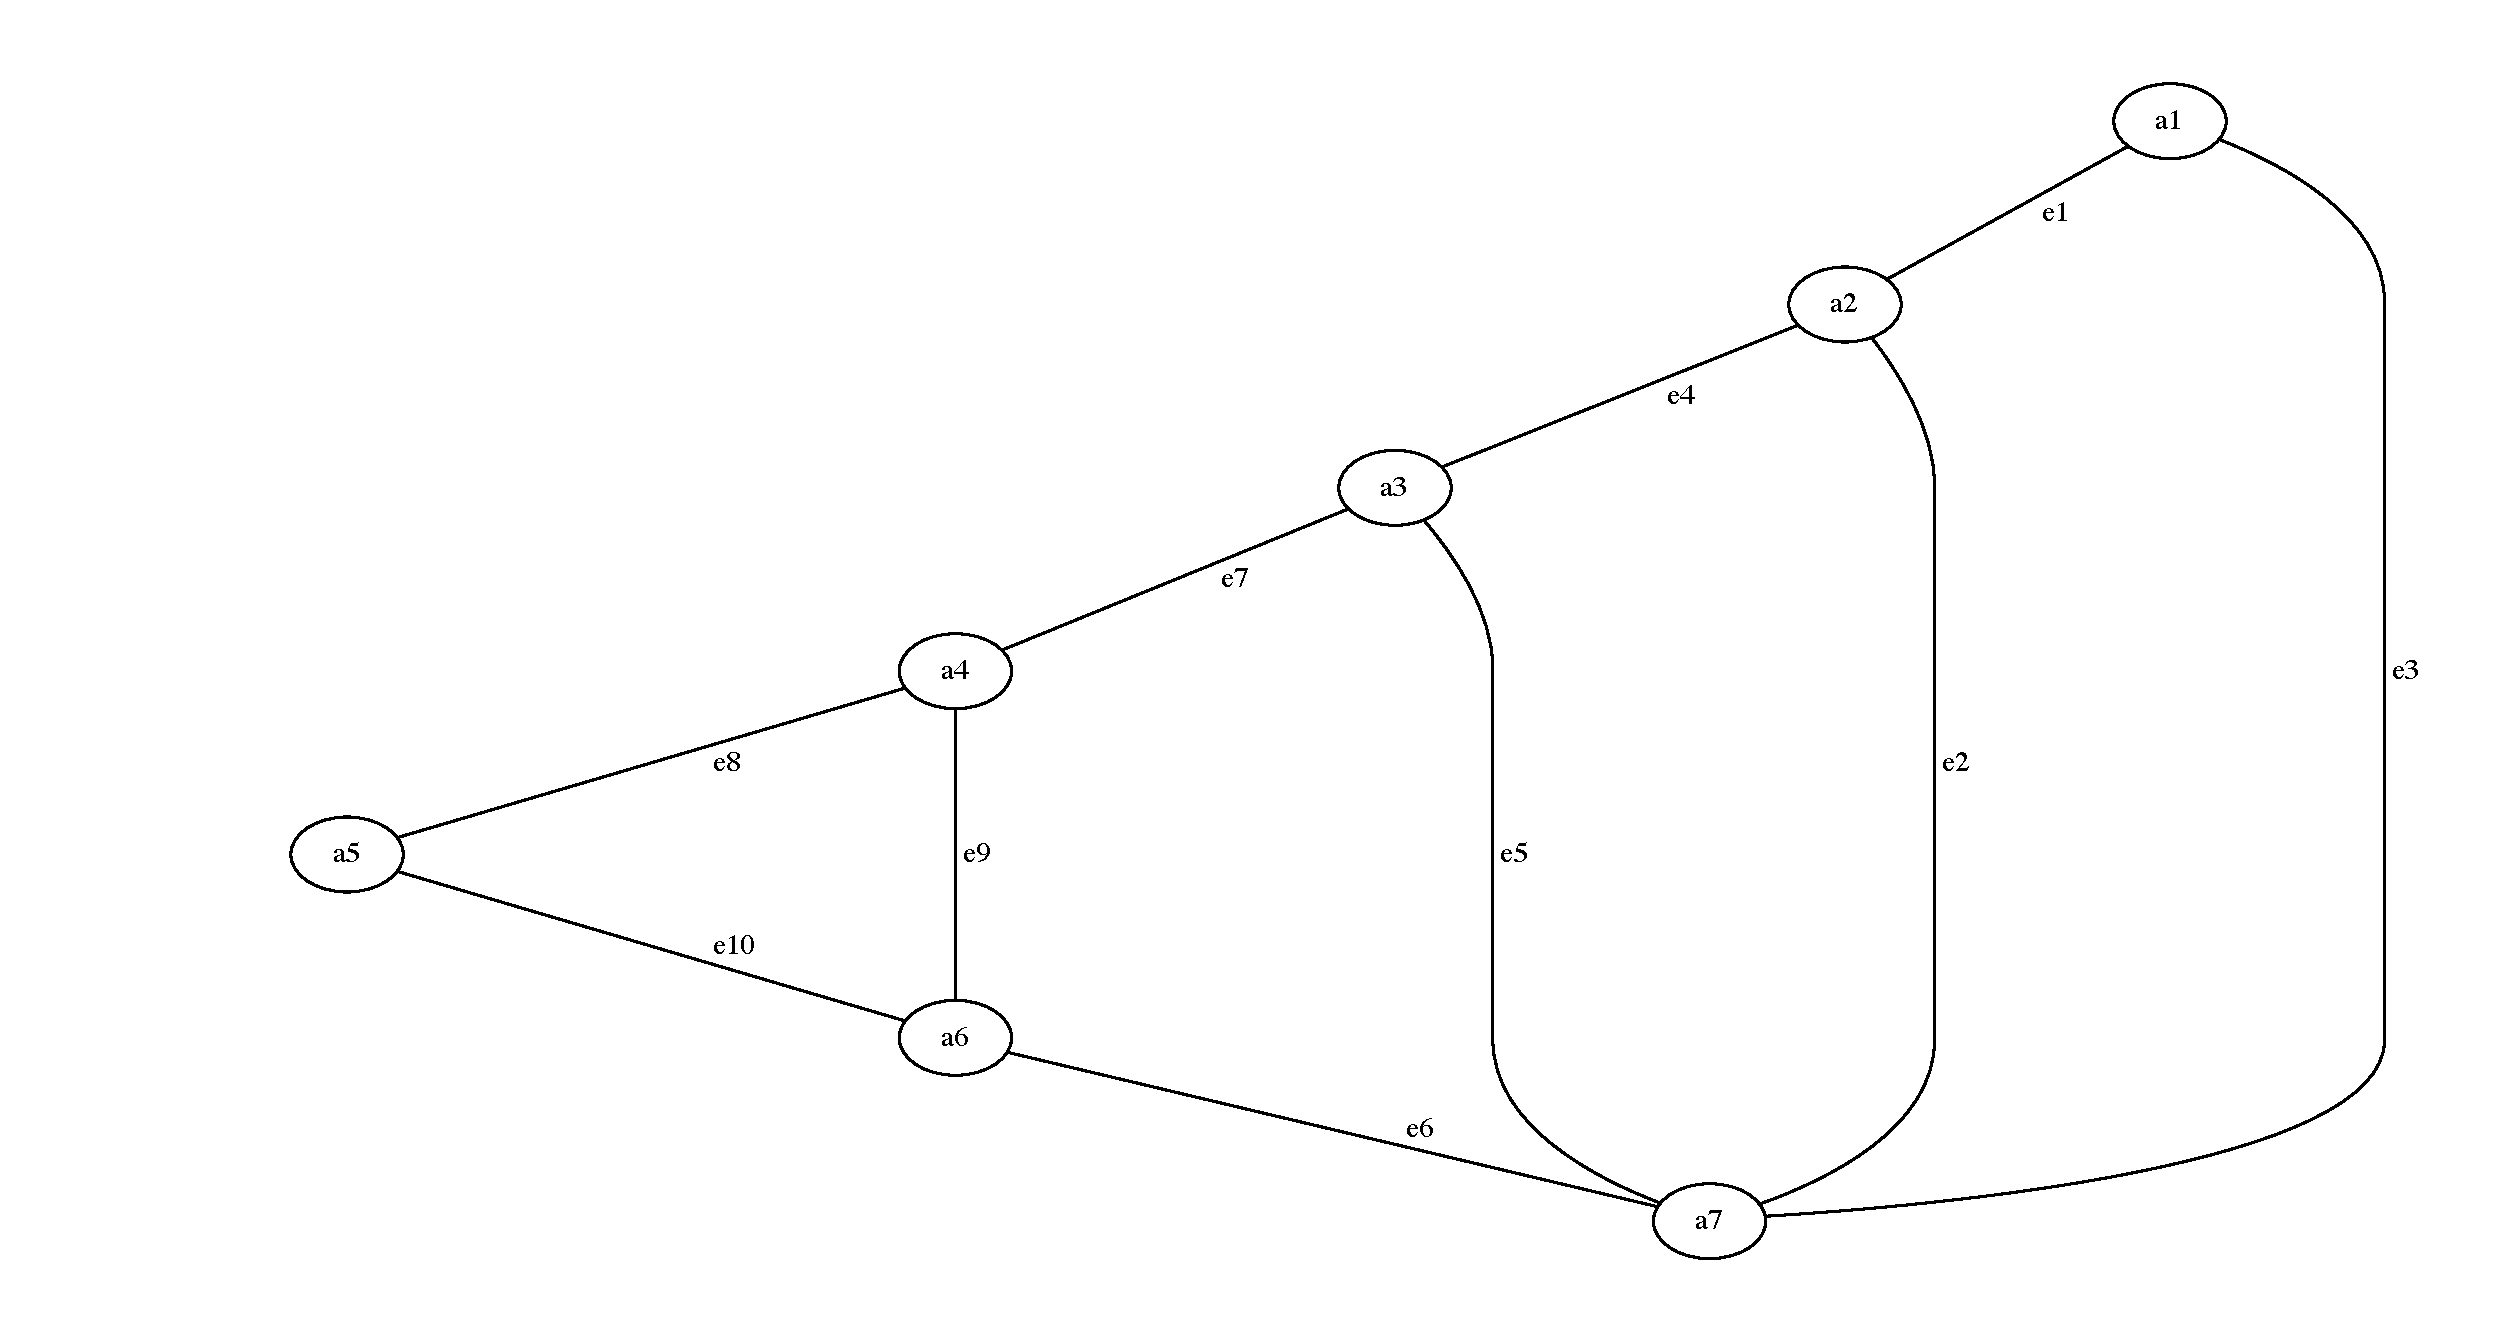
\includegraphics[scale=0.35]{diagrams/Chapter4_Example1.pdf}\\
\end{example*}
Remark: Perfect matching not possible with $\lvert V \rvert$ being odd. 
Maximum cardinality = 3. Empty set is a matching. All subsets of matchings are matchings.
\\
Maximum cardinality:
$\left\{e_{3},e_{1},e_{9}\right\}$
 $\left\{e_{10},e_{5},e_{1}\right\}$\\
Maximal matching:
$\left\{e_{2},e_{9}\right\}$
\begin{lemma}
If $M$ is a matching of maximum cardinality it is a maximal matching.
\end{lemma}
\begin{proof}
Let $M'$ be a matching with $M\subseteq M'$, assume $M \subset M'$ then $\lvert
M' \rvert > \lvert M \rvert \Lightning \:$(as $M$ has maximum cardinality).
\end{proof}
Remark: There are maximum matchings without maximum cardinality.
\begin{lemma}
If $M$ is perfect then $2 \lvert M \rvert = \lvert V \rvert$.
\end{lemma}
\begin{proof}
Obvious.
\end{proof}
\begin{lemma}
If a graph has a perfect matching $M$ then every matching of maximum cardinality is perfect. Clearly, $M$ is
of maximum cardinality.
\end{lemma}
\begin{proof}
Obvious.
\end{proof}
\section{Matching in bipartite graphs}\index{Matching in bipartite graphs}
Problem: Find a matching of maximum cardinality in a bipartite graph.\\
Solution: Construct an associated network as follows:\\
Let $G=(V,E)$ in a bipartite graph.\\ $V = X \cup Y$\\$\overline{V}=V \cup \left\{s,t\right\}$\\
$X\cap Y=\emptyset$\\$\overline{E}=\left\{s \rightarrow x: x \in X \right\}\cup \left\{ y \rightarrow t: y \in Y \right\}$\\
$\overline{c}(\overline{e})=1, \forall \overline{e} \in \overline{E}$
\begin{example*}
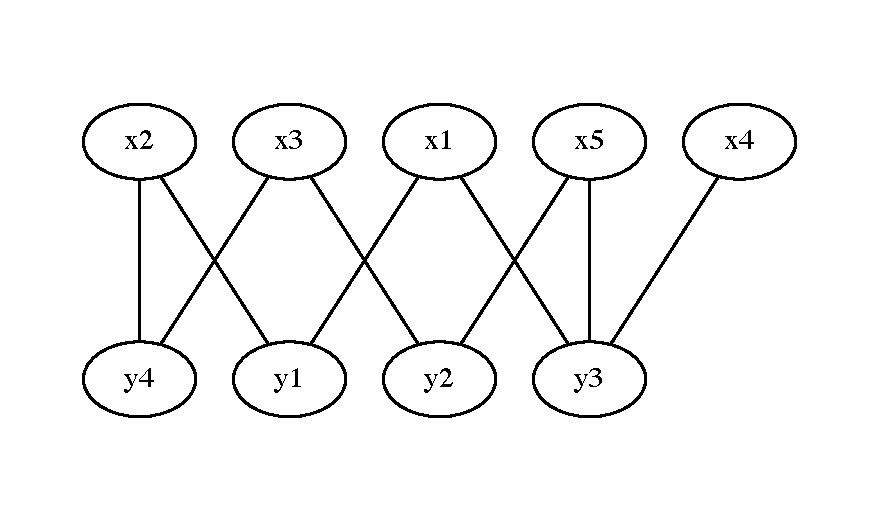
\includegraphics[scale=0.7]{diagrams/Chapter4_Example2.pdf}\\
One solution:\\
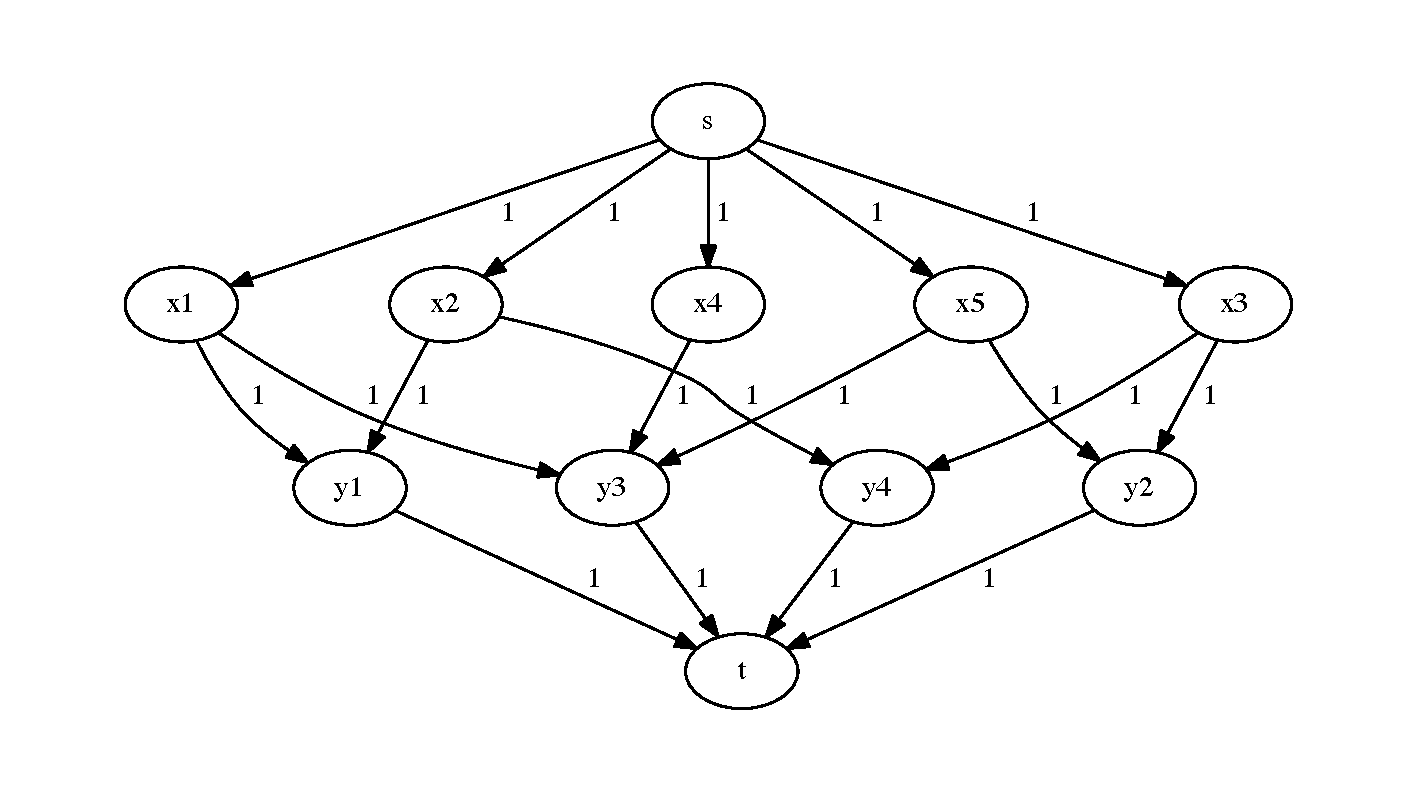
\includegraphics[scale=0.7]{diagrams/Chapter4_Example3.pdf}\\
\begin{enumerate}
  \item $s$ marked
  \item $x_{1}: \overrightarrow{(s, x_{1})}$
  \item $x_{2}: \overrightarrow{(s, x_{2})}$
  \item $x_{3}: \overrightarrow{(s, x_{3})}$
  \item $x_{4}: \overrightarrow{(s, x_{4})}$
  \item $x_{5}: \overrightarrow{(s, x_{5})}$
\end{enumerate}
Solution:\\
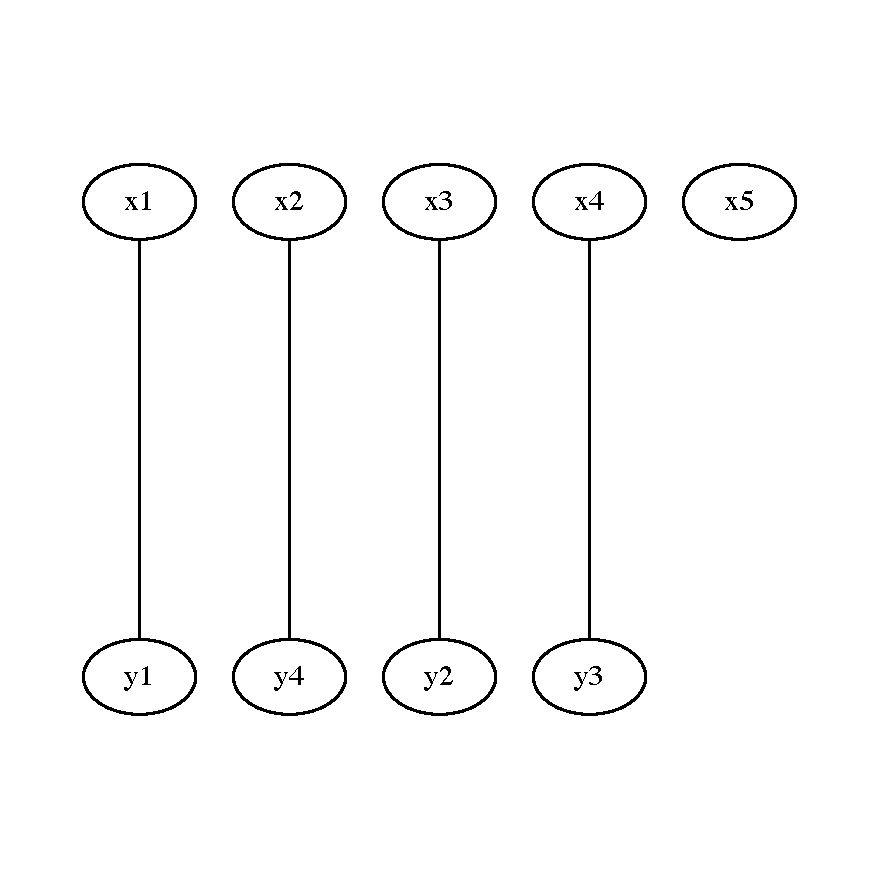
\includegraphics[scale=0.7]{diagrams/Chapter4_Example12.pdf}\\
\end{example*}
\begin{theorem}
The number of edges in a matching $M$ of maximum cardinality coincides with $F_{max}$, i.e. the
 maximum total flow in the associated network.
\end{theorem}
\begin{proof}
Let $M$ be a matching of maximum cardinality. For every edge $x-y$ in $M$ we transport one unit along
the path $s-x-y-t$. We can do that as the edges in $M$ are node disjoint, i.e. they do not share nodes.
This defines a flow function $f'$ with $F'=\lvert M \rvert$ and hence $F_{max}\ge F' = \lvert M \rvert$. 
Now let $f$ be an arbitrary flow function for the associated network, without loss of generality we may choose
$f$ such that $f(e)\in \mathbb{N} \: \forall e$. All paths that connect $s$ with $t$ have the form 
$s \rightarrow x \rightarrow y \rightarrow t$. If such a path is used to transport a unit value then it is clear that
no flow can happen along edges of the form $x \rightarrow y'$ or $x' \rightarrow y$.
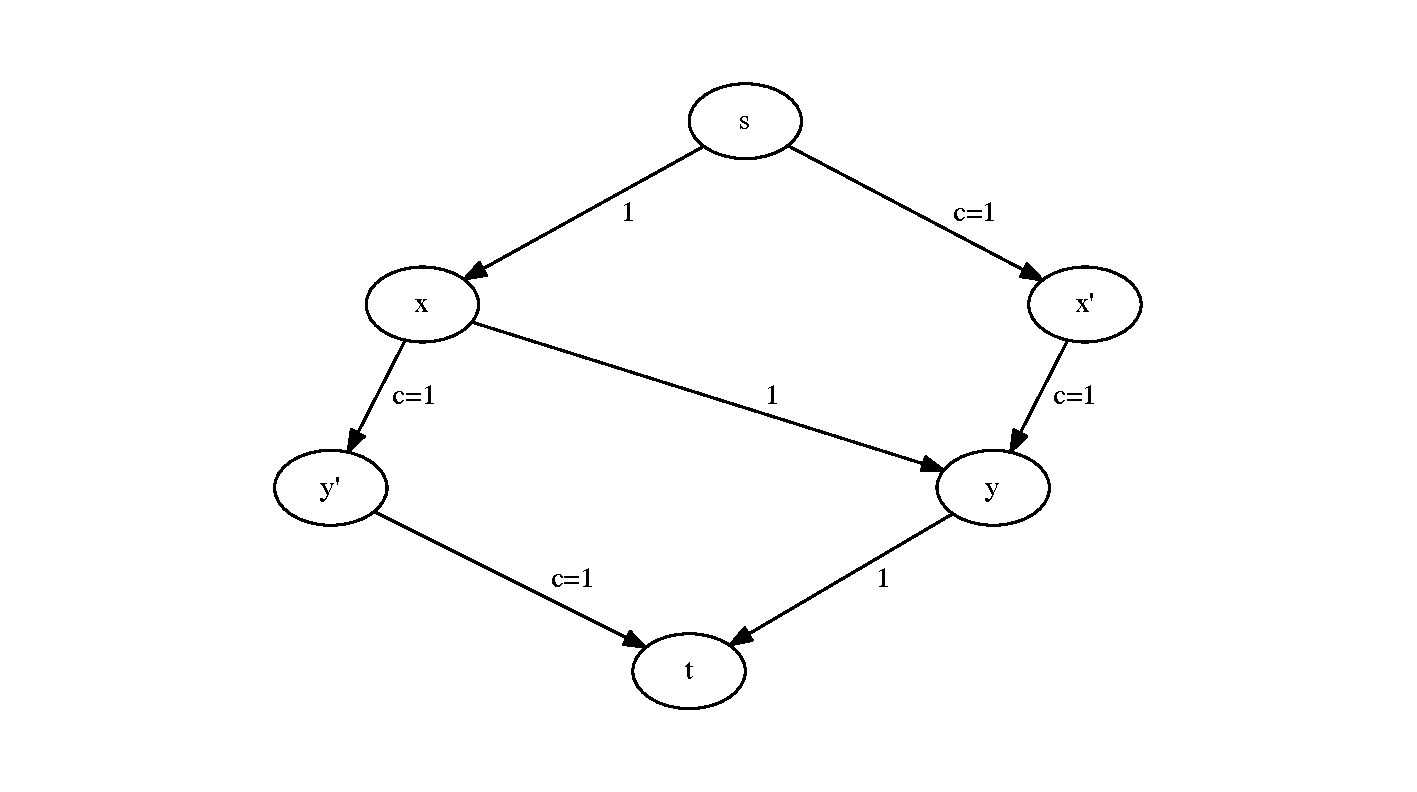
\includegraphics[scale=0.7]{diagrams/Chapter4_Example4.pdf}\\
Let $N=\left\{x-y:f(x \rightarrow y)=1\right\}$. $N$ is a matching and the total flow of $f$, i.e. $F$, satisfies
$F=\lvert N \rvert \le \lvert M \rvert$, hence also $F_{max}$, because $M$ was assumed to be of maximum cardinality.
Hence $\lvert M \rvert=F_{max}$ because we chose $f$ arbitrarily. 
\end{proof}
This theorem yields an algorithm to determine
a matching of maximum cardinality. Given a bipartite graph $G=(V,E)$ with $V = X
\cup Y$ and $X \cap Y = \emptyset$:
\begin{enumerate}
  \item Construct the associated network.
  \item On this network, calculate a flow function with maximum total flow.
  \item The matching of maximum cardinality is obtained by $N=\left\{x - y: f(x \rightarrow y) = 1\right\}$.
\end{enumerate}
\begin{definition}
Let $G$ be a bipartite graph, $V = X \cup Y; \: X \cap Y = \emptyset$. Let $A
\subseteq X$. Let $\Gamma(A)= \left\{y \in Y: \exists x \in A: x - y \in E\right\}$. ($\Gamma(A)$: potential partners for the elements in A).
A matching $M$ is called \emph{complete} if $\lvert M \rvert = \lvert X \rvert$, i.e. every $x \in X$ gets a partner.
\end{definition}
\begin{theorem}
Wedding or marriage theorem: A bipartite graph has a complete matching if and only if for every $A \subseteq X$
$\lvert \Gamma(A) \rvert \ge \lvert A \rvert$.
\end{theorem}
\begin{proof}
``>'' Let G have a complete matching $M$, let $A \subseteq X$. Then every $x \in X$ has a partner for itself in $M$,
hence for every $A \subseteq X \lvert \: \Gamma(A) \rvert\ge \lvert A \rvert$. \\
``<'' Let $\lvert \Gamma (A) \rvert \ge \lvert A \rvert$ for every $A \subseteq X$. Assume there is no complete
matching. Let $S$ be the set of nodes that were marked in the last step of Ford-Fulkerson in the associated 
network. The calculated flow function determines a matching $M$ with i) $F=\lvert M \rvert$. As we assumed that there
is no complete matching we get ii) $\lvert M \rvert < \lvert X \rvert$.\\
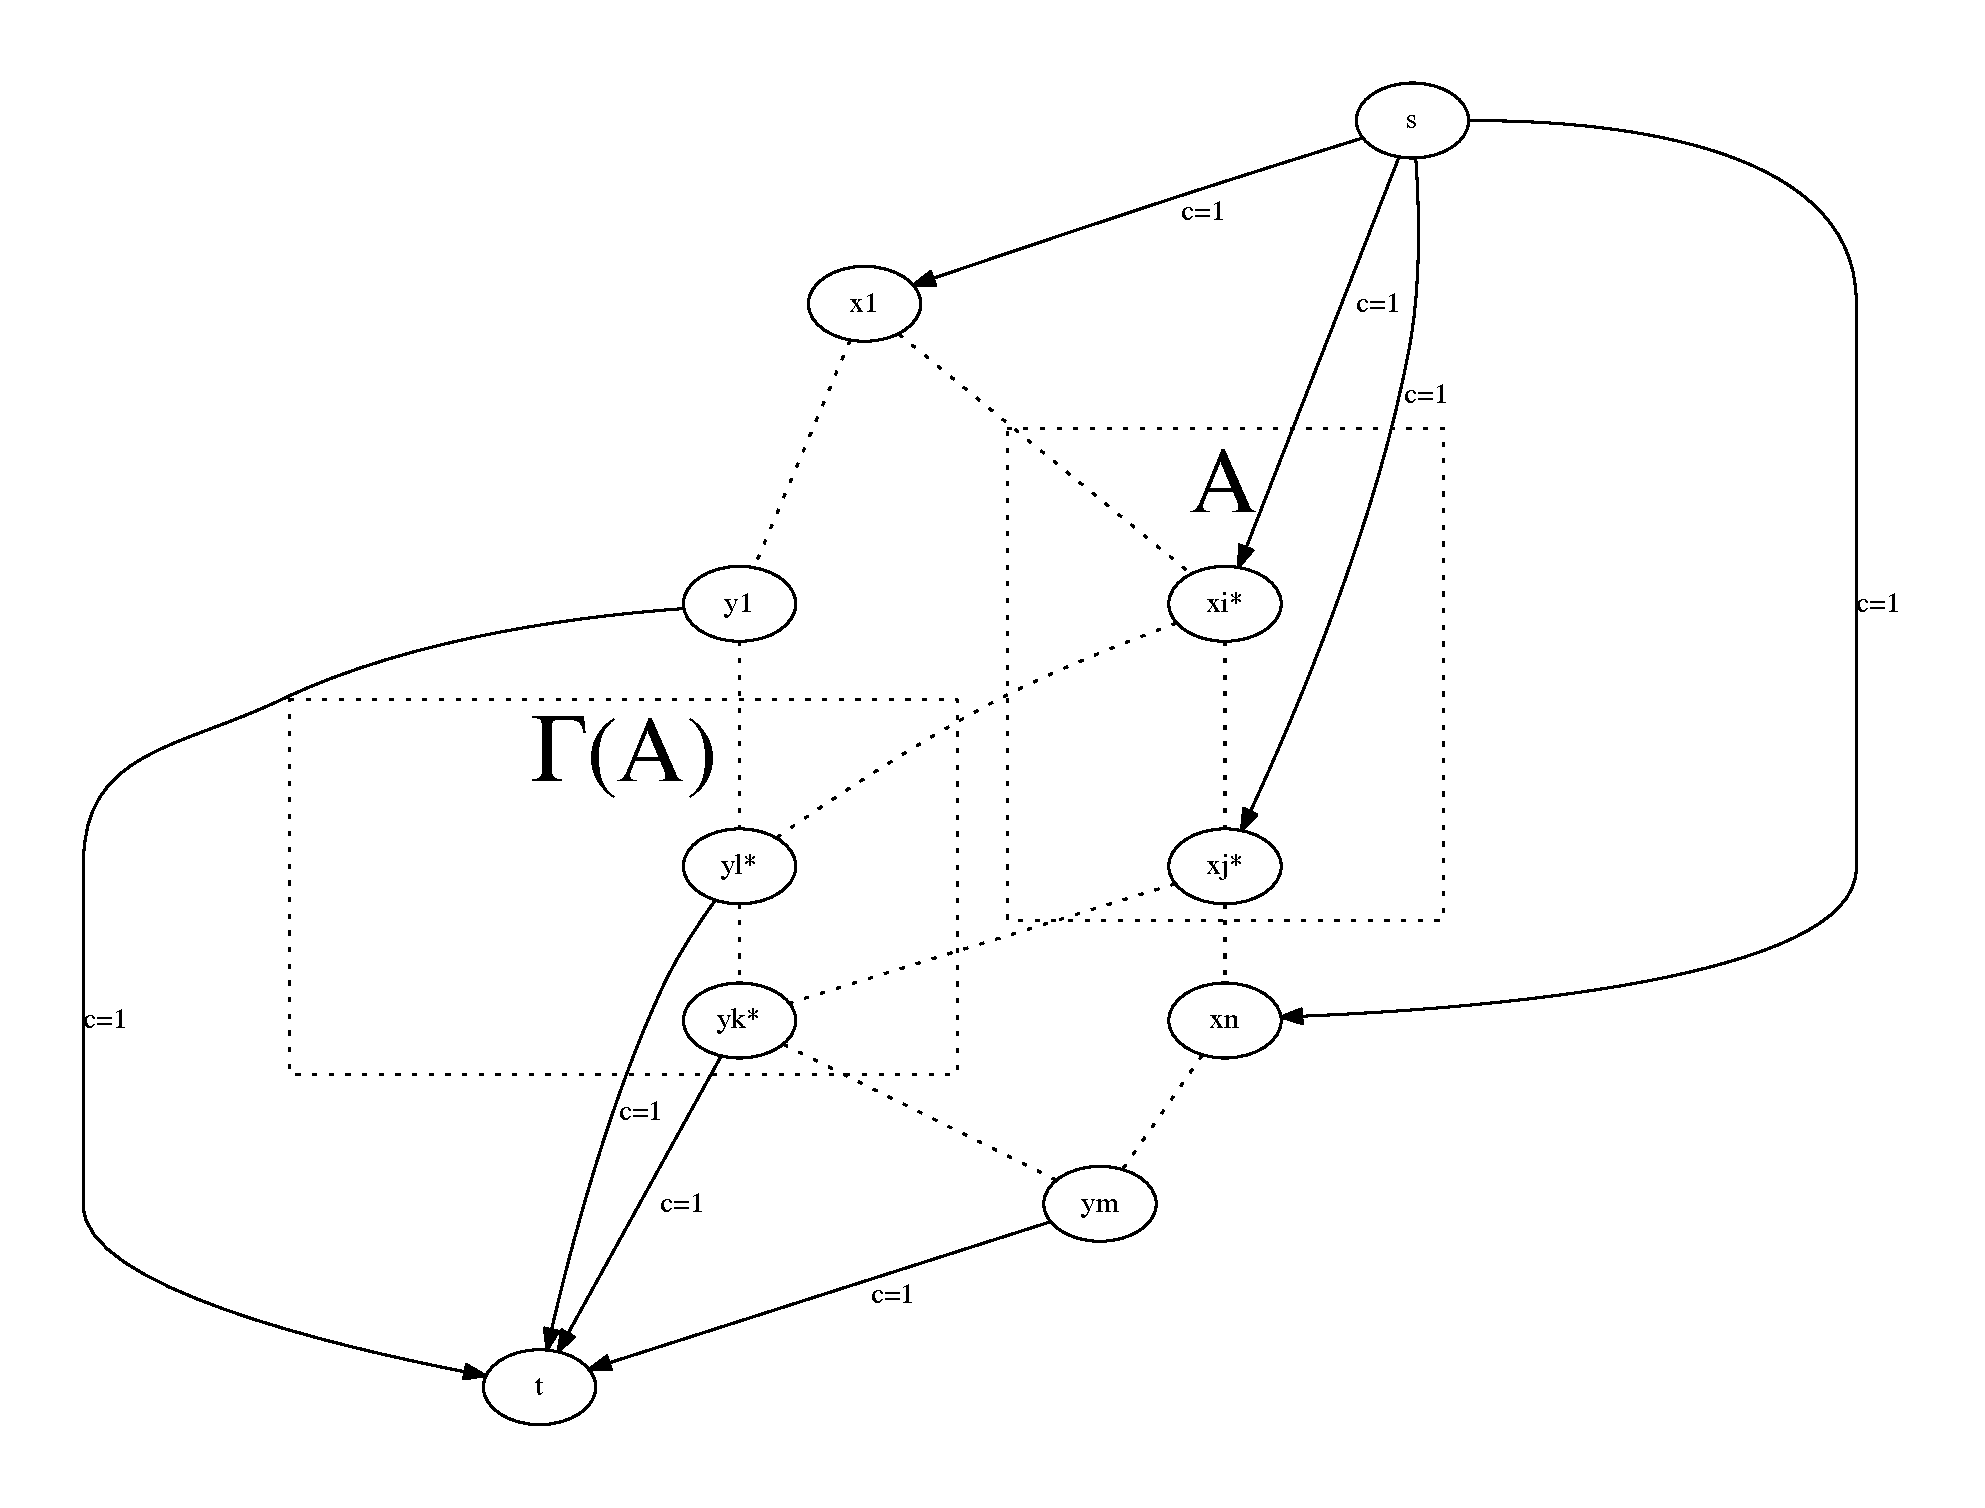
\includegraphics[scale=0.45]{diagrams/Chapter4_Example5.pdf}\\
Marking in the last round of Ford-Fulkerson. $S=$ the marked nodes.\\
$A:=X \cap S$\\
Let $y \in \Gamma (A)$ then there is an $x \in A = \: X \cap S \: x$ marked and $x-y$ is an edge in $E$.\\
In the last successful construction of an augmenting path there was no flow determined along the edge $s \rightarrow x$,
otherwise we could not mark $x$ now. Hence the flow along the edge $x \rightarrow y$ must have been $0$ before 
as well. Hence the remaining capacity $x \rightarrow y \: = 1$.
\section{Stable matching (marriage)}\index{Stable matching (marriage)}
Given:\\ 
1. n men $b_{1} \dots b_{n}$, n women $a_{1} \dots a_{n}$\\
2. each person has a preference list of the other sex: \\
$a_{1}: b_{2}, b_{3}, b_{1} \dots$, where $a_{1}$ likes $b_{2}$ best.
\end{proof}
Task: Form couples respecting the preferences.\\
A matching or coupling associates with each man exactly one woman. A matching is called \emph{unstable} if there is a man $a$ and a woman $A$ such that:
$a$ prefers $A$ to the woman $B$ he is matched with and $b$ prefers $B$ to the woman $A$ he is matched with.
A matching is called \emph{stable} if it is not unstable.\\
Given n men, n women. Here are two approaches:\\\\
\underline{1. Attempt: Try all possible matchings}\\
%[INSERT MISSING ILLUSTRATION!]
There are $n!$ possible matchings. There are therefore ${n \choose k} =
O(n^2)$ checks to find out if one given matching is stable altogether $O(n! * n^2)$.
For n=10 this equals 300,000,000 checks.\\\\
\underline{2. Gale-Shapley Algorithm}
\begin{enumerate}
\item{Mark every person as ``free''.}
\item{As long as there is a free man m do: Let F be the first woman to which m has not yet made an offer. If F is 
free then match m with F ((F,m)) and mark both as ``bound''. If F is bound to m' then check if F prefers
m to m'. If this is so, substitute the pair (F, m') by (F.m). Mark m' as free and m as ``bound''.\\If F does not
prefer m to m' then nothing is changed.}
\item{Output all pairs.}
\end{enumerate}
\underline{Statement:} For any input the algorithm terminates and yields a
stable matching.\\
\emph{1. Observation:} It cannot happen that a man is rejected by all
women.
This is because if a woman rejects or leaves a man she is bound.
When the man reaches the end of his list then all women would be bound.
\Lightning because there are $n$ women and $n-1$ other men. \\
\emph{2. Observation:} The algorithm consists of offers made by men. Each
man makes at most n offers $\implies O(n^2)$ offers in the worst case. \\
\emph{3. Observation:} The result is a matching because the algorithm
terminates when all men are bound and every man is bound to exactly one woman. \\
\emph{4. Oberservation:} The resulting matching is stable. Assume this is
not the case.\\
$m$: $F' \dots F$ \\
$F'$: m \dots m' \\
$F$ matched with $m$. \\
$F'$ matched with $m'$. \\
m makes offers according to his list. So he made an offer to F' before he
reached F.\\
\emph{Case 1}: $F'$ was free. So she accepted his offer, but later
left him.
This can only happen because of men she likes better than $m$, but $m'$ could not break
into such a marriage. \\
\emph{Case 2}: $F'$ was bound. \\
\emph{Case 2.1}: $F'$ was bound to a partner she prefers to $m$,
then she does not leave this partner because of $m$ and def. not because of $m'$.\\
\emph{Case 2.2}: $F'$ leaves her partner because of $m$, but $m'$
cannot break into this marriage. \\
Hence the matching is stable. The cost of the algorithm is $O(n^2)$. \\
$n=10$: algorithm takes 100 Steps; trying all takes 300,000,000 steps. \\
$n=1009$: algorithm takes $10^6$ steps;  trying all takes $500^500$ steps. Age
of planet earth: $4*10^9$ years.\\
A man and a woman $F$ are called \emph{stable partners} if there is a stable
matching in which they are bound to each other. \\
\emph{Statement:} All executions of the algorithm yield the same result. In this
matching each man gets the best partner he can get in any stable matching. Let E
be an arbitrary execution of the algorithm, let the result be the matching
$M_{E}$. Assume there is another matching $M$.\\
$M_{E}$: $m - F$ \\
$M$: $m - F'$ \\
$m$: $\dots F' \dots F \dots$ \\
Then deriving $E$, $F'$ must have rejected / left $m$. Without loss of
generality, let this be the first time that a woman rejected / left a stable
partner. Let $m'$ be the reason for this.\\
$F'$: $\dots m' \dots m \dots$ \\
Then $m'$ cannot have a stable partner he prefers to $F'$, hence $m'$ prefers
$F'$ to his partner in $M$.\\
$M$: $m - F'$; $m' - F''$\\
So $M$ is not stable.

\section{Maching in general graphs}
\label{sec:Matching in general graphs}
 \begin{example*}
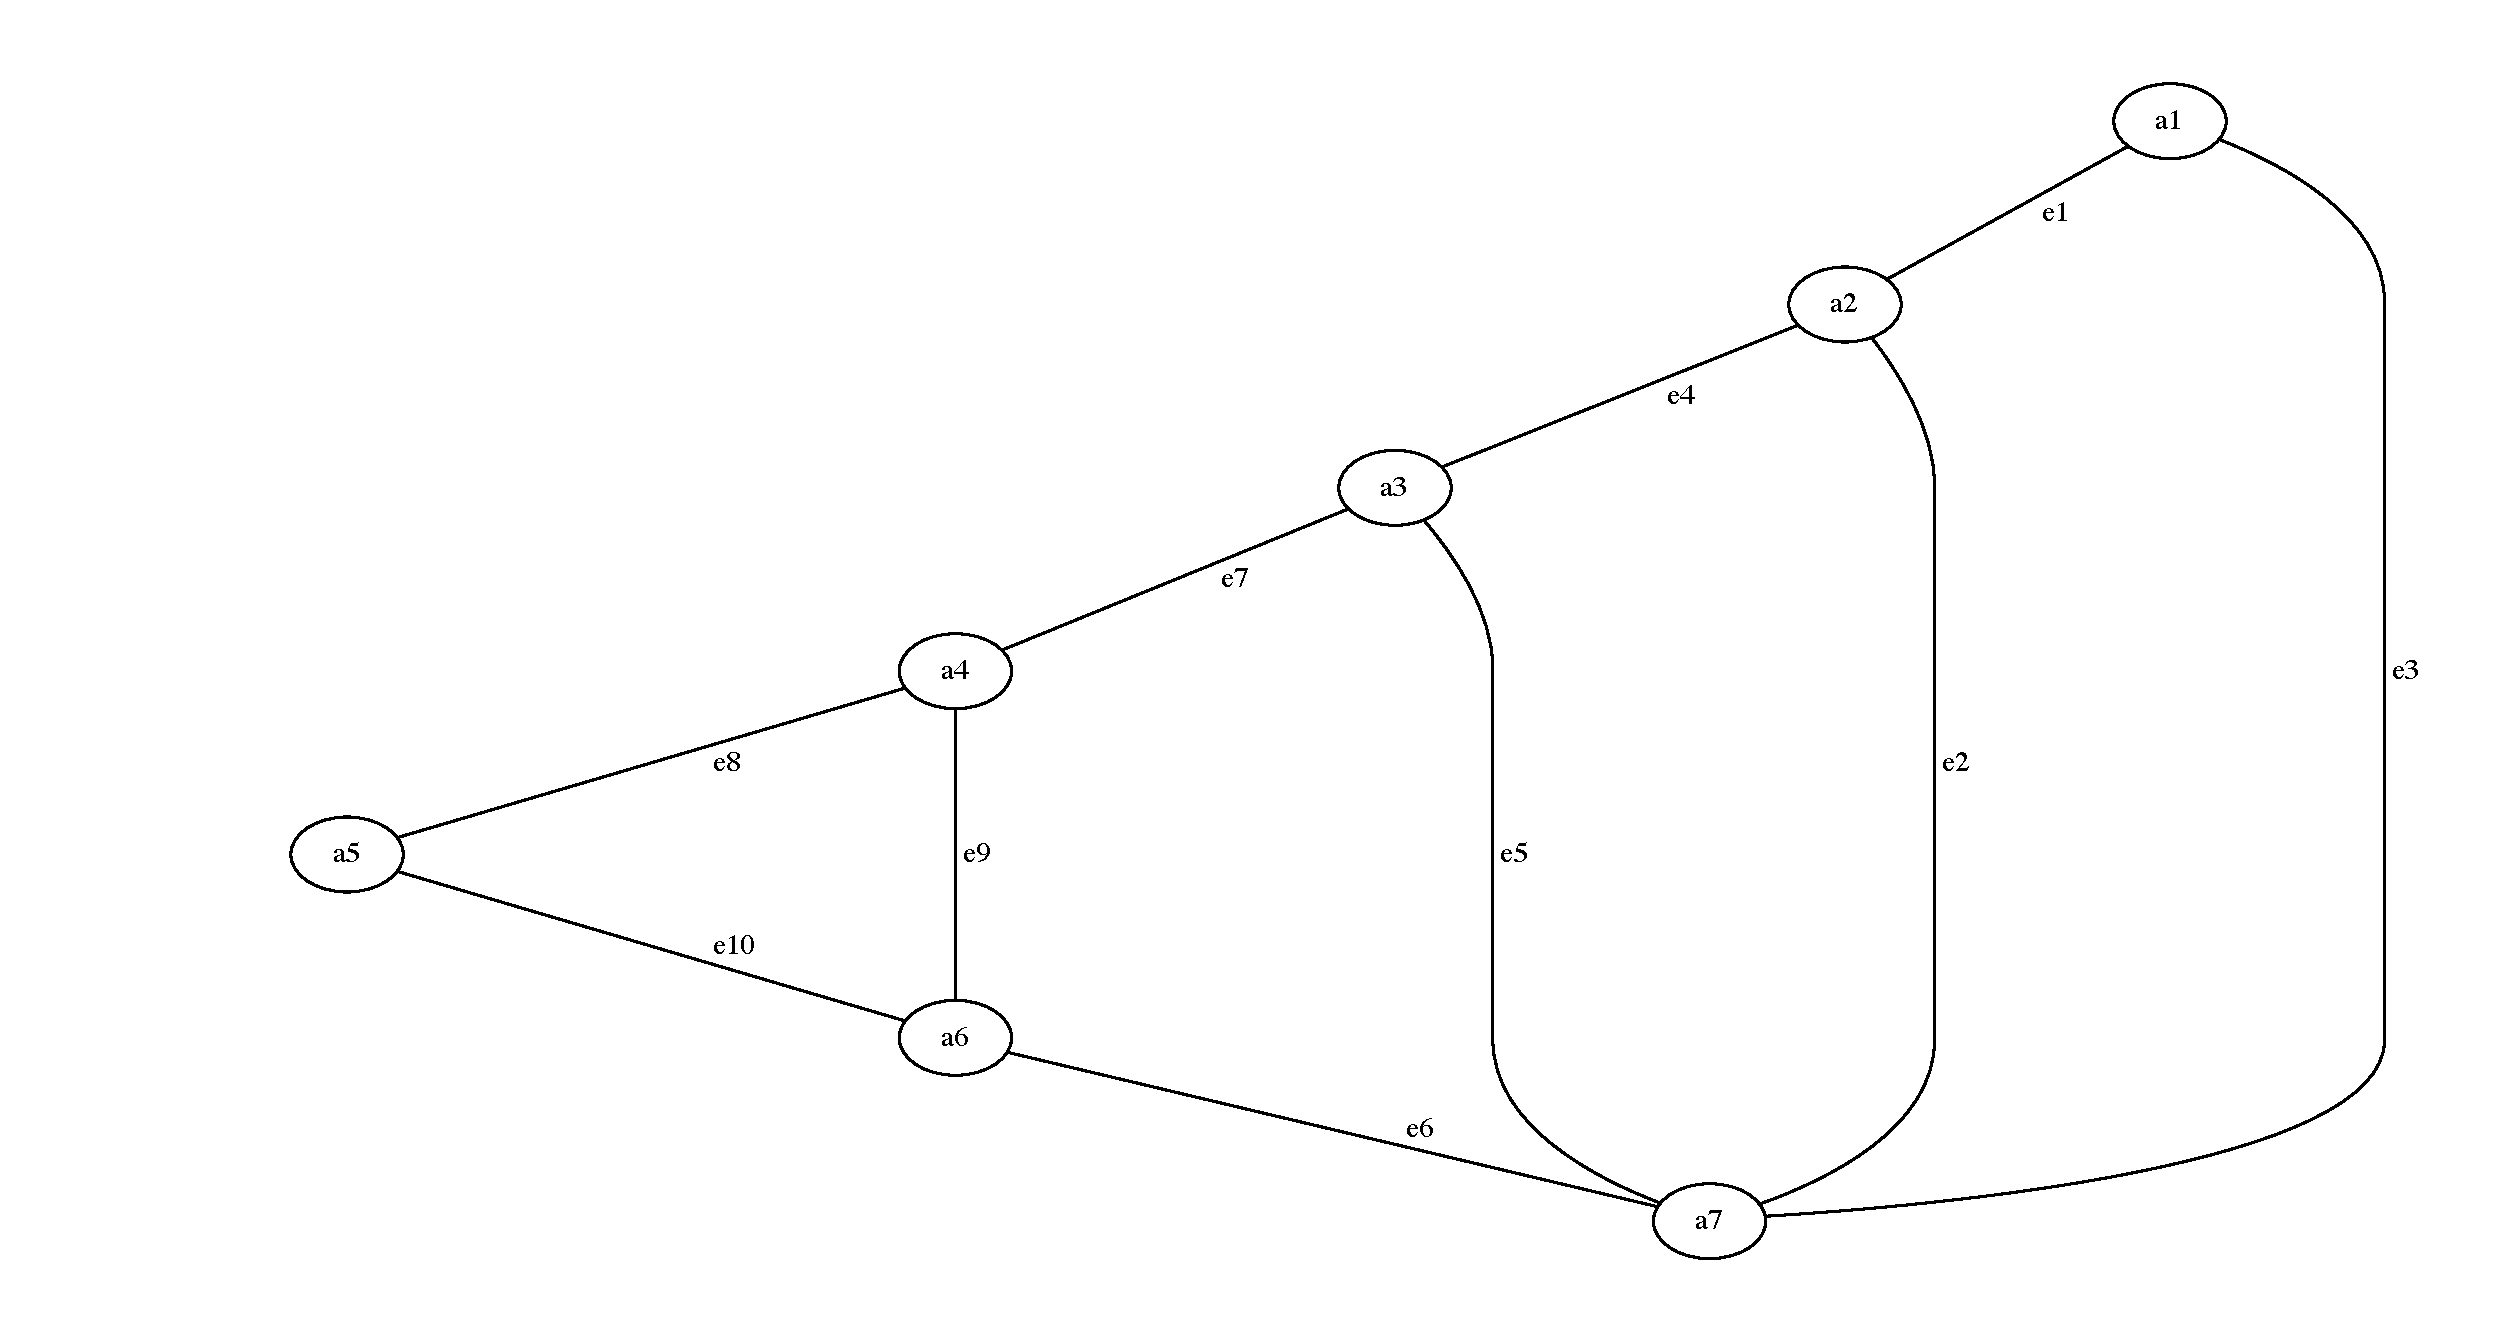
\includegraphics[scale=0.35]{diagrams/Chapter4_Example1.pdf}\\
\end{example*}
$\{e_{1}, e_{5}, e_{9}\}, \: \{ e_{1}, e_{5}, e_{10}\}$ are both matchings of
maximal cardinality because $|V|=7$.\\
Every subset of a matching is a matching.
\begin{example*}
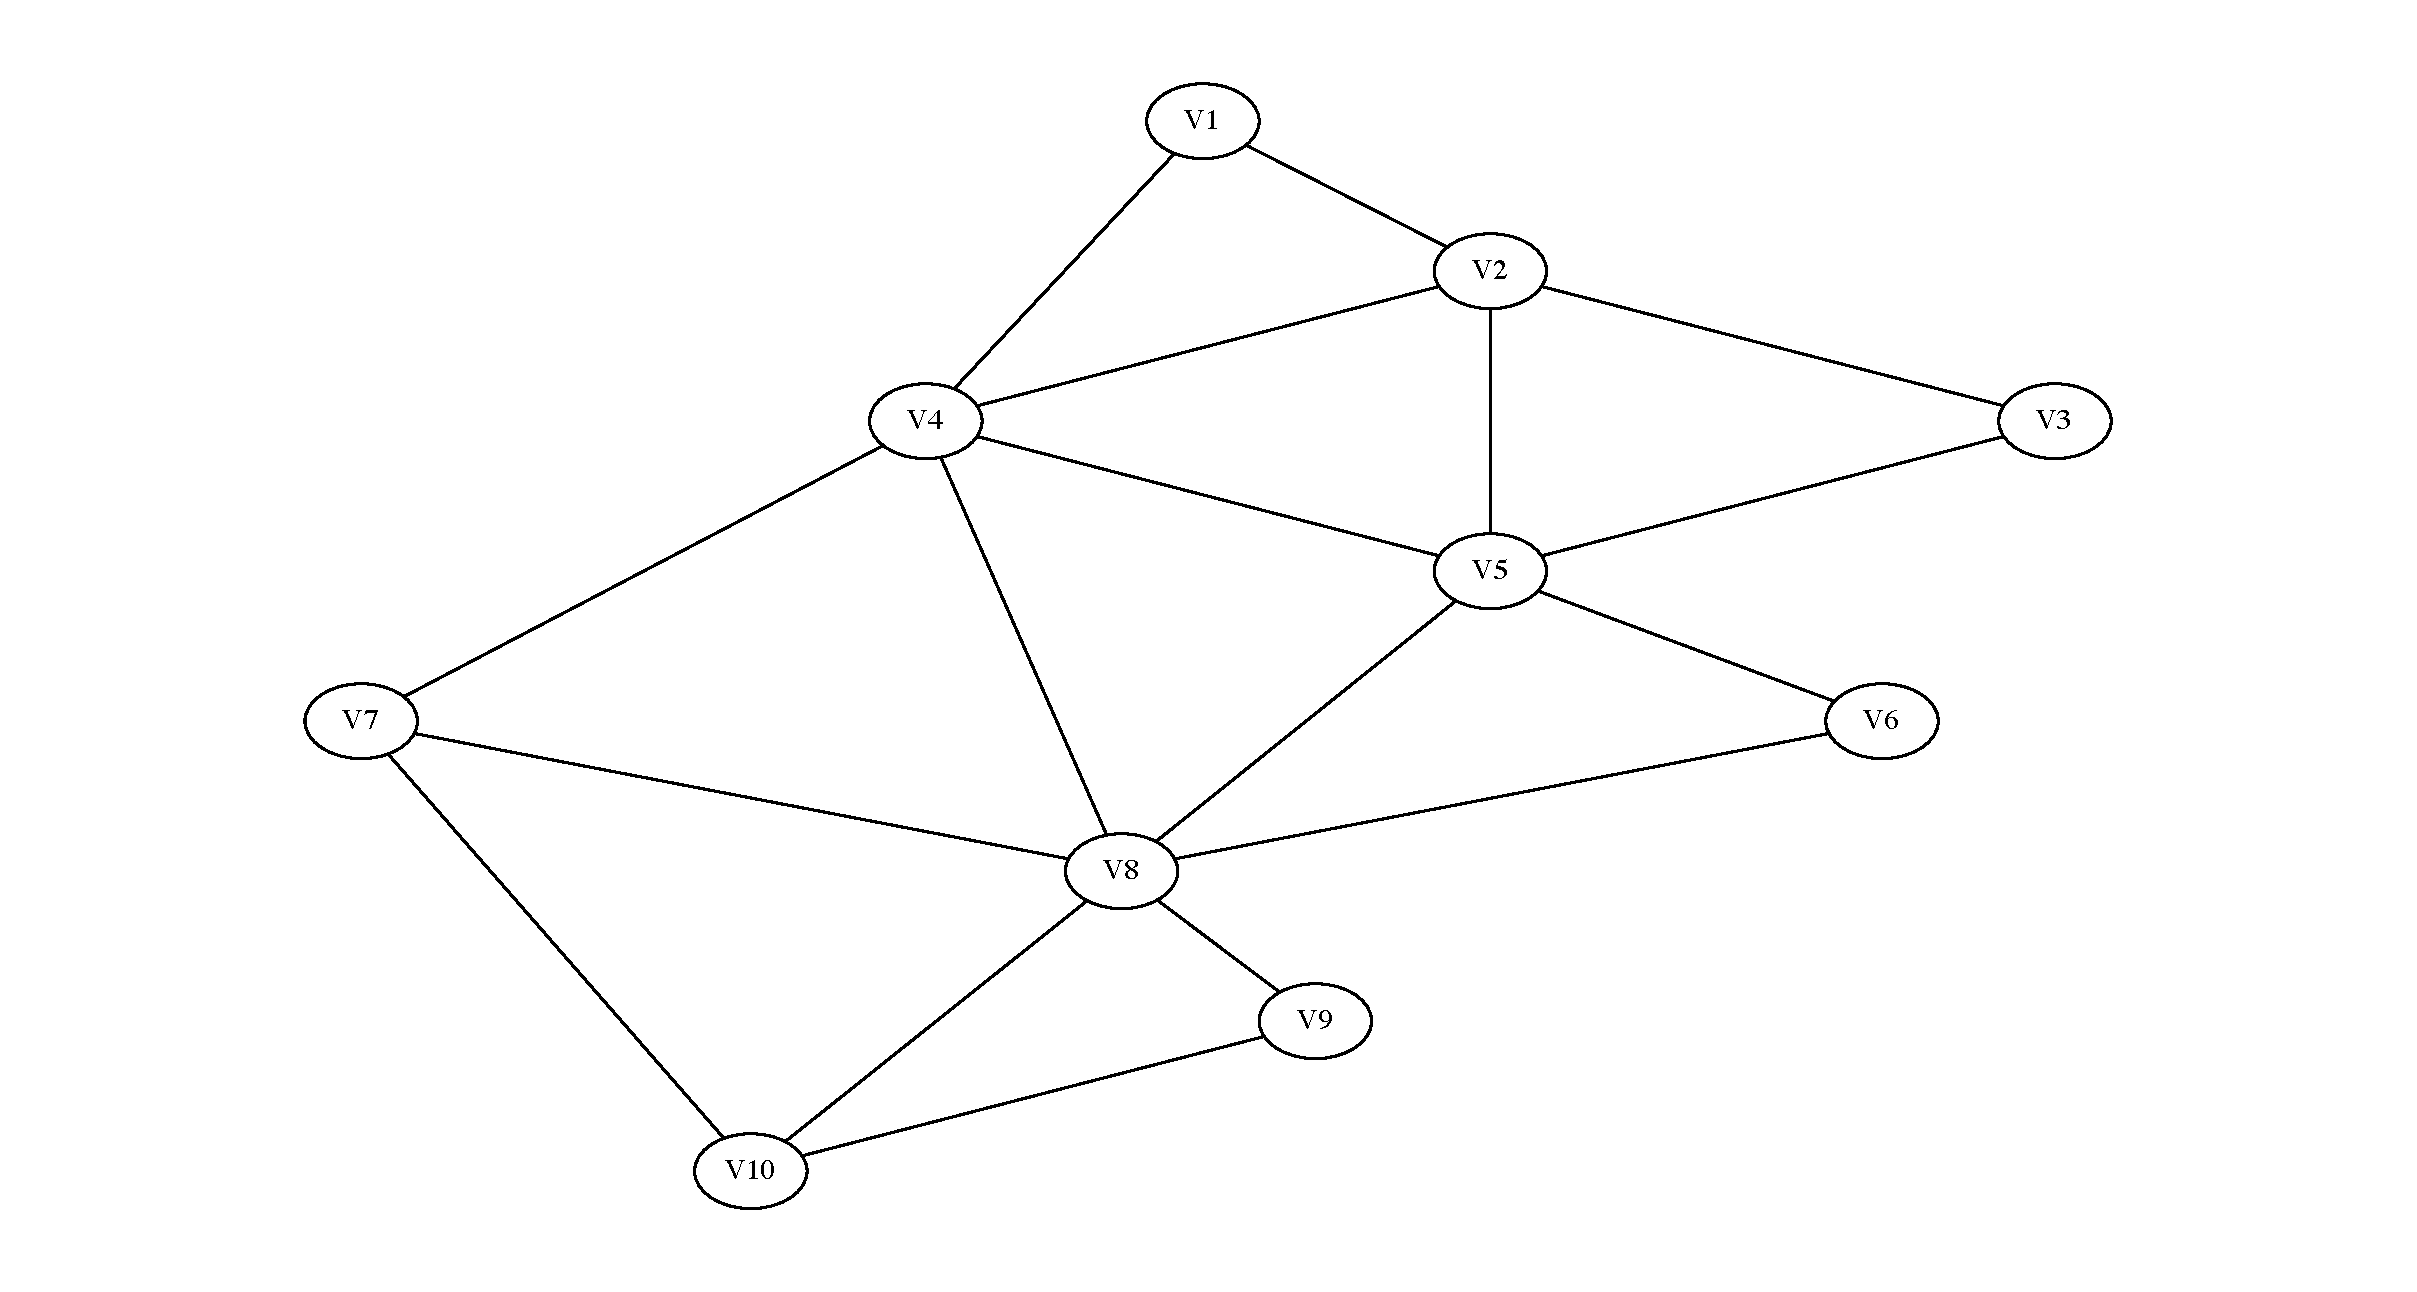
\includegraphics[scale=0.35]{diagrams/Chapter4_Example6.pdf}\\
\end{example*}
$M_0=\{\{V_{2}, V_{3}\}, \{V_{4}, V_{5}\}, \{V_{7}, V_{10}\}\}$
\begin{definition}
	Let $G=(V,E)$ be a graph and $M$ a matching for $G$. The edges in $M$ are
	called ``matched'', the others are called ``free''. If $\{u,v\} \in M$ then
	$u,\:v$ are called partners and ``matched''. If $v \in V$ lies on no edge of
	$M$ then $v$ is called ``free''. A simple path $e_{1}, e_{2}, \dots, e_{k}$ is
	called $M$-alternating if $e_{1}, e_{3}, e_{5} \dots$ are free eges and
	$e_{2}, e_{4}, \ldots$ are matched.\\
		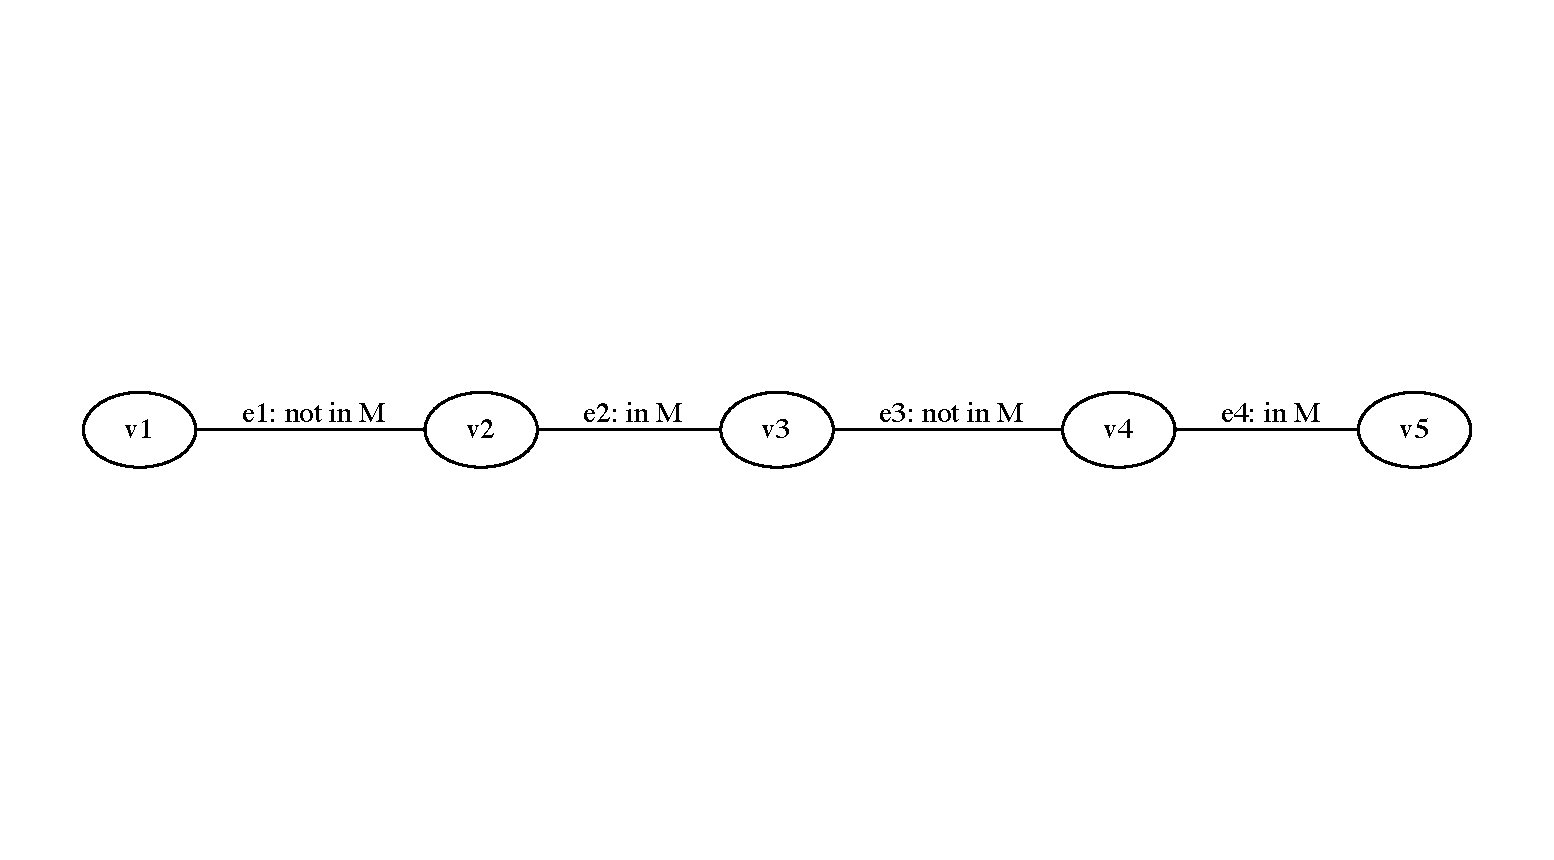
\includegraphics[scale=0.5]{diagrams/Chapter4_Example7.pdf}\\
		\\
	An $M$-alternating path is called $M$-augmenting if the start and end points of
	the path are free.
\end{definition}
\begin{lemma}
	If p is an $M$-augmenting path, $p=e_{1}, \dots, e_{l}$, then $l$ is odd and
	the number of nodes in the path is even.
\end{lemma}
\begin{proof}
	As the first and last node on an $M$-augmenting path must be free, the first
	and last edge must be free edges.\\
	$\frac{e_{1}}{free} \: \frac{e_{2}}{free} \: (e_{1} \: e_{2})(e_{3} \: e_{4})
	\dots$ \\
	Assume $l$ is even, then we can group the edges into pairs $ (e_{1} \:
	e_{2})(e_{3} \: e_{4}) \dots$ and so on and the last edge would then be
	matched.\\ \emph{Contradiction:} In a simple path of odd length the number of
	nodes is even.\\
\end{proof}
\begin{lemma}
	Let $G=(V,E)$ be a graph, $M$ a matching and $p$ an $M$-augmenting path. Then
	$M'=M \smallsetminus p \cup p \smallsetminus m$ is a matching and $|M'| =
	|M|+1$.
	(See ex. $E$ and $M_{0}$). \\
\end{lemma}
\begin{itemize}
	\item{$p=v_{6} - v_{8}$\\$M_{0}$-alternating? Yes \\$M_{0}$-alternating? Yes}
	\item{$p'=v_{1} - v_{2}$\\$M_{0}$-alternating? Yes \\$M_{0}$-alternating? No}
	\item{$M_{1} = M_{0} \smallsetminus p \cup p \smallsetminus M_{0} = \{\{v_{2}, v_{3}\},
	\{v_{4}, v_{5}\}, \{v_{7}, v_{10}\}, \{v_{6}, v_{8}\}\}$}
	\item{$p_{1}: v_{1} - v_{2} - v_{3} - v_{5} - v_{4} -
	v_{8}$\\$M_{1}$-alternating? Yes \\ $M_{1}$-alternating? No}
	\item{$p_{2}: v_{1} - v_{4} - v_{5} - v_{6} - v_{8} -
	v_{7} - v_{10} - v_{9}$\\$M_{1}$-alternating? Yes \\ $M_{1}$-alternating? Yes}
	\item{$M_{1} = M_{1} \smallsetminus p_{2} \cup p_{2} \smallsetminus M_{1} = \{\{v_{2},
	v_{3}\}, \{v_{1}, v_{4}\}, \{v_{5}, v_{6}\}, \{v_{8}, v_{7}\}, v_{10},
	v_{9}\}\}$}\\ $|M_{2}| = 5$ is of maximum cardinality as there are 10 nodes.
\end{itemize}
\begin{proof}
Let $p$ be an $M$-augmenting path. \\$p$: $v_{1} - v_{2} - v_{3} \dots -
v_{2k}$\\
Show 1. $M'$ is a matching $(M' = M \smallsetminus p \cup p \smallsetminus M)$, i.e. no two
edges share a node. Assume there are two edges in $M'$ that share a node, $e$
and $e'$. There are 3 cases to consider:\\
i) $e, e' \in M \smallsetminus p$ \\
ii) $e, e' \in p \ M$  \\
iii) $e \in M \smallsetminus p, e' \in p \smallsetminus m$ \\
\emph{Case i)} $e, e'$ share a node and are in $M \smallsetminus p$, in particular $e,
e' \in M \: \lightning $ \\
\emph{Case ii)} $e, e' \in p \smallsetminus M$, in particular $e, e' \in p$ and not in
$M$. But on $p$ only edges share a node if one is in $M$ and the other isn't. \\
\emph{Case iii)} Let $e \in M \smallsetminus p, \: e' \in p \smallsetminus M$,
i.e. $e'$ is free. 
\begin{example*}
		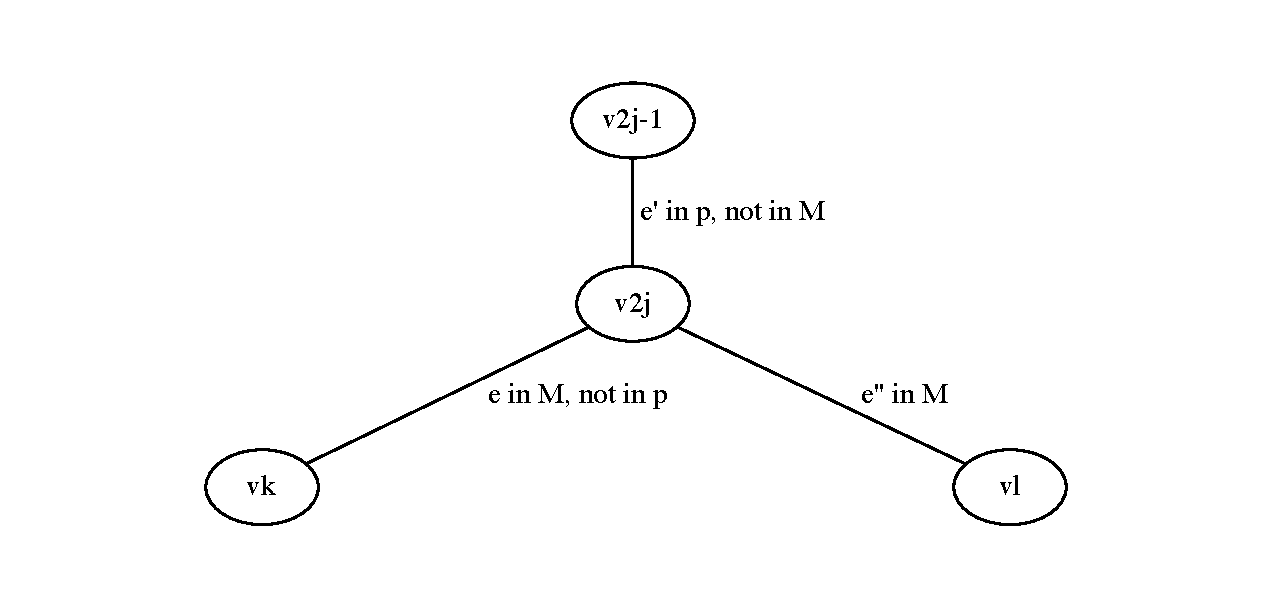
\includegraphics[scale=0.65]{diagrams/Chapter4_Example8.pdf}\\
\end{example*}
Without loss of generality, assume that $v_{2j}$ also lies on $e$. \\
$e''$ is in $M$, hence $e, e'' \in M$ and share a node. $\lightning$. (If
$v_{2j}$ is the last node, use $v_{2j-1}$ for a similar argument.) \\
Show 2. $|M'| = |M| + 1$ \\
$p$: $v_{1} - v_{2} \dots v_{2k-1} - v_{2k}$, where $\{v_{1}, v_{2}\}$ and
$\{v_{2k-1}, v_{2k}\}$ are not in $M$. \\
$p$ contains $2k-1$ edges and $k-1$ belong to $M$ and $k$ do not belong to $M$.\\
$e_{1}, e_{3}, \dots, e_{2k-1}$ \\
$|(M \smallsetminus p) \cup (p \smallsetminus m)| = |M \smallsetminus p| + |p \smallsetminus M|\\ =
|M| - (k-1) + k \\ = |M| + 1$\\
\end{proof}
\begin{lemma}
	$G=(V,E)$ graph, $M$ matching, $u\in V$ free. Let us assume that there is no
	$M$-augmenting path starting in u. Let $p$ be an $M$-augmenting path with end
	points $v, w$. Then there will be no $(M \smallsetminus p \cup p \smallsetminus
	)$-augmenting path starting from $u$.
\end{lemma}
\begin{lemma}
A matching $M$ is of max. cardinality if and only if there is no $M$-augmenting
path.
\end{lemma}

\begin{proof}
``>'' Let $M$ be of max. cardinality. Assume there is an augmenting path, then
construct $M'=M \smallsetminus p \cup p $ and $|M'| > |M| \lightning$. \\
``<'' Let there be no $M$-augmenting path. Assume that there is a matching $M'$
with $|M'| > |M|$. Consider the edges in $M \smallsetminus M' \cup M' \smallsetminus M$.
$G' = (V, (M \smallsetminus M') \cup (M' \smallsetminus M))$. In this graph every node has 
degree 2 or less. If $v$ has degree 2, then one edge belongs to $M$, the other
to $M'$. Two connected components of $G'$ are either paths or circles. \\
		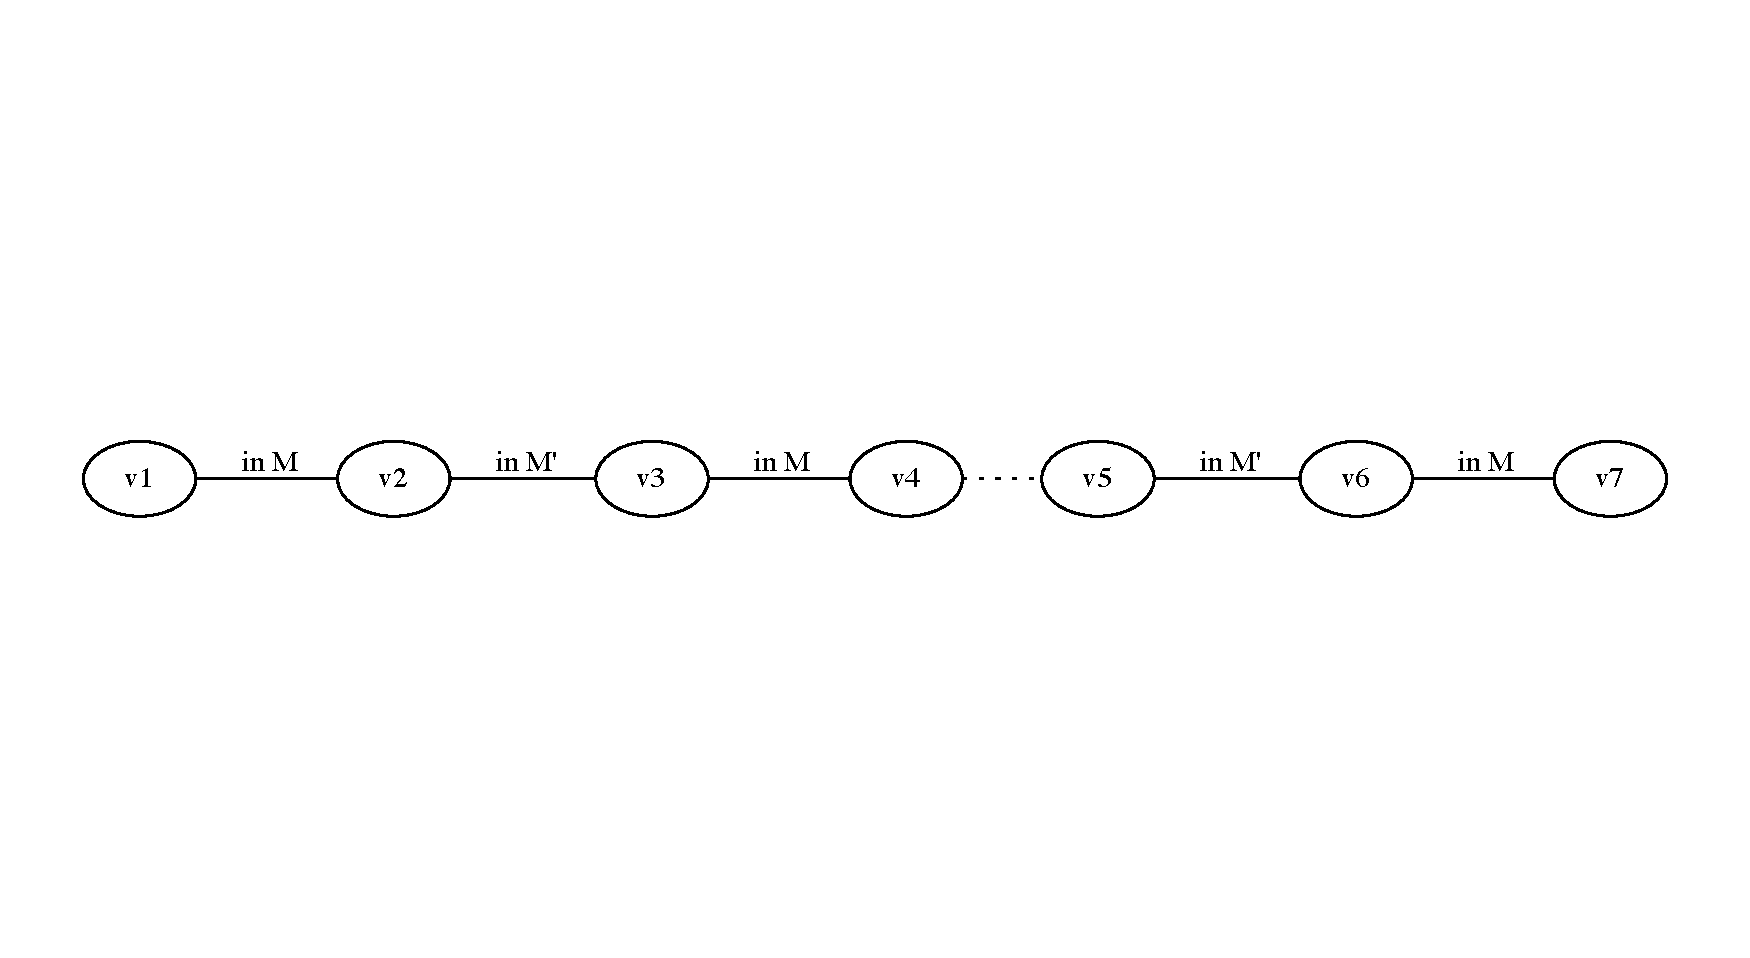
\includegraphics[scale=0.5]{diagrams/Chapter4_Example9.pdf}
\\or\\
		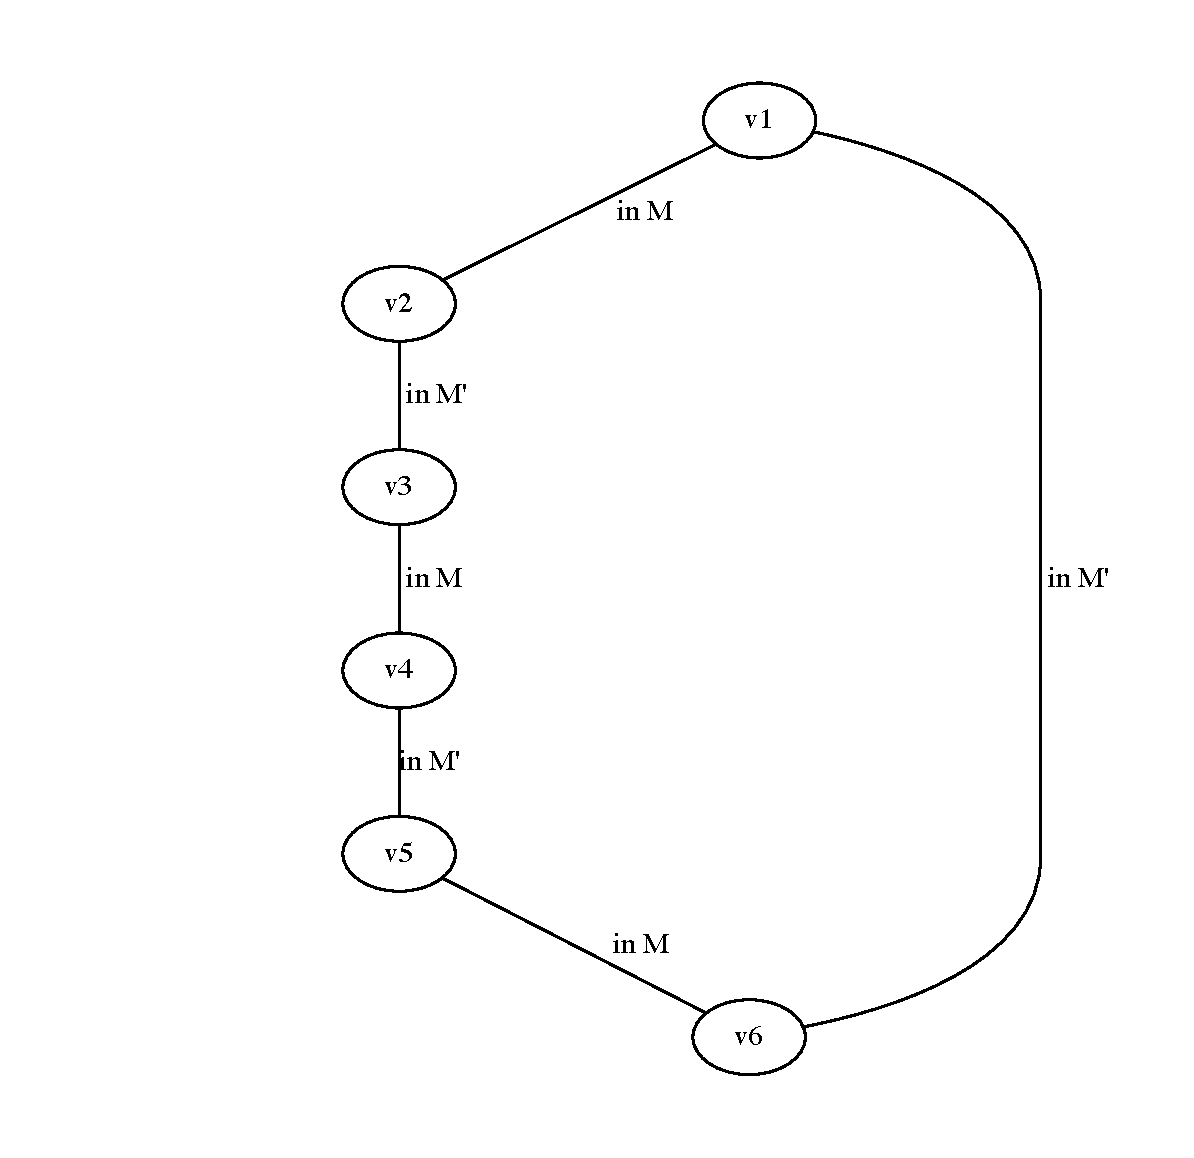
\includegraphics[scale=0.5]{diagrams/Chapter4_Example10.pdf}\\
where the number of edges in the circle belonging to $M$ equals the number of
edges
belonging to $M'$. As $|M'| > |M|$ and the circle cannot contribute to this
fact, we conclude that there must be a path with more edges in $M'$ than in $M$.
This path must look like this:
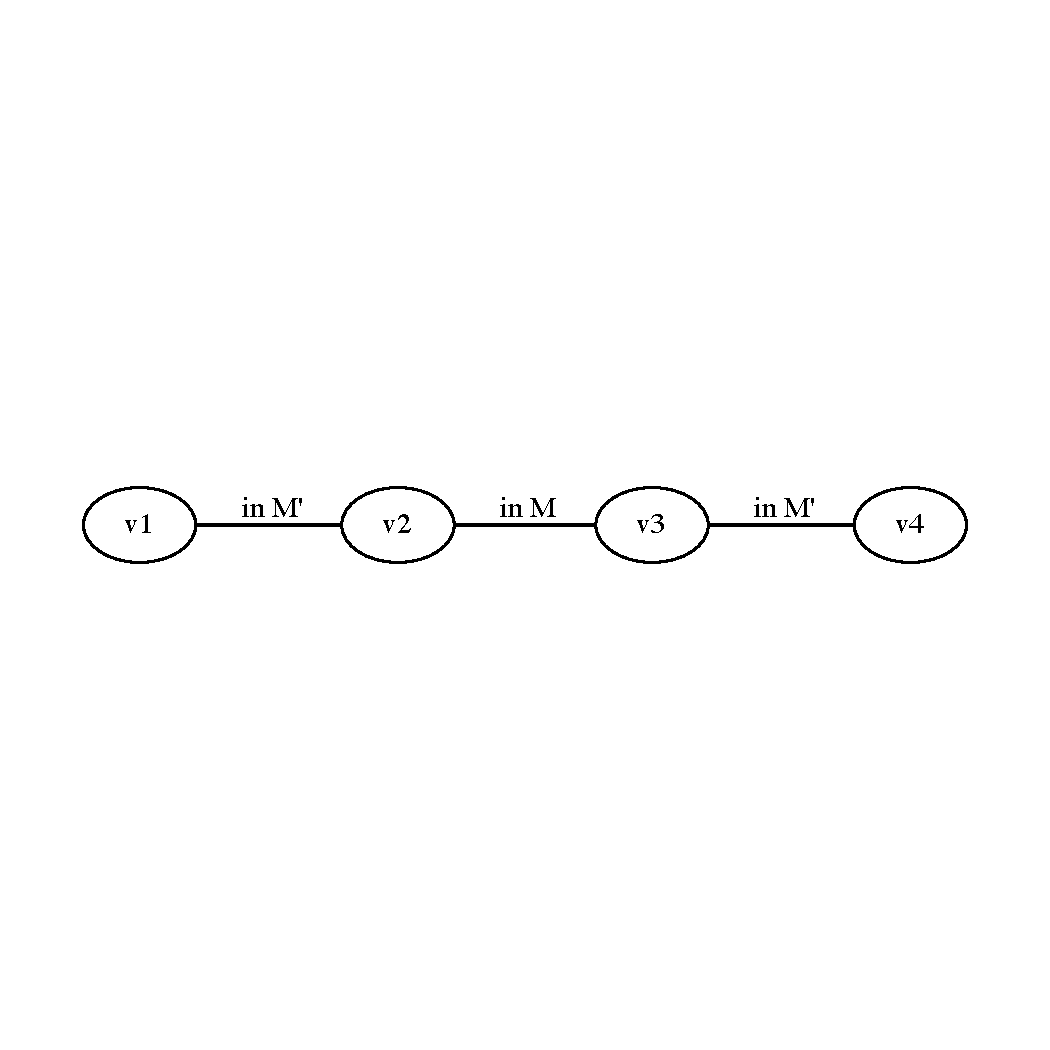
\includegraphics[scale=0.5]{diagrams/Chapter4_Example11.pdf}\\
$\lightning$
\end{proof}
Here is an idea for an algorithm which finds a matching of maximal cardinality:
\begin{enumerate}
  \item {Start with an initial matching, e.g. consisting of one edge}
  \item {Find an M-augmenting path. Put $M = M \smallsetminus p \cup p \smallsetminus
  M$. Go to 2. If there is no M-augmenting path, stop; the current matching is
  of maximal cardinality.}
\end{enumerate}
